\documentclass{sem5}
\usepackage{caption}
\institutename{Indian Institute of Information Technology, Vadodara}
\author{Dilip Puri}
\idt{201351014}
%\team{teamname}
\collab{\textbf{Collaborators} - Hemant Kumar(201352026)\\ Govind Meena(201352010)}

\coursename{Parallel Programming}
\ccode{\begin{small}CS403\end{small}}
\profname{Prof. Reshmi Mitra}

\type{Project}
\typeid{1}
\submissiondate{\today}%dd/mm/yyyy
\deadline{Sep12, 11.59 PM}%dd/mm/yyyy @hh:mm pm/am
\problemset{LU Decomposition}

\begin{document}

\section{Introduction}
Suppose we have the system of equations
\begin{center}AX=B\end{center}
Even most of the mathematical model follows these kind of systems. The motivation for an LU decomposition is based on the observation that systems of equations involving triangular coefficient matrices are easier to deal with.  Indeed, the whole point of Gaussian Elimination is to replace the coefficient matrix with one that is triangular.  The LU decomposition is another approach designed to exploit triangular systems. We suppose that we can write
\begin{center}A = LU\end{center}
where L is a lower triangular matrix and U is an upper triangular matrix. Our aim is to find L and U and once we have done so we have found an LU decomposition of A.
Let A be a square matrix. If there is a lower triangular matrix L with all diagonal entries equal to 1 and an upper matrix U such that A=LU, then we say that A has an LU-decomposition. It can be helpful in calculating various types of operation on matrices. Here L matrix has the upper triangular values as 0 and U has lower triangular values as 0 and diagonal values same as that of the original matrix. 

\section{Algorithm}

To decompose matrix A into L and U we are using Doolittle's method which is described as follows
\begin{figure}[htbp]
\centering
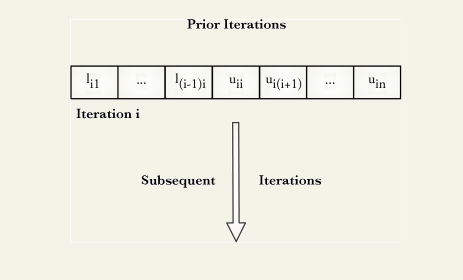
\includegraphics[scale=.5]{1.png}
\caption{Computational Sequence of Doolittle's Method}
\end{figure}
\begin{figure}
\centering
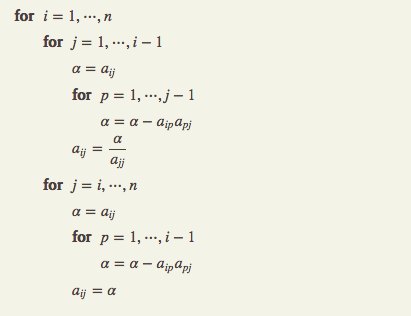
\includegraphics[scale=.5]{2.png}
\caption{Doolittle's LU Decompostion Algorithm}
\end{figure}
\newpage
\section{Serial Code}
\lstinputlisting[frame=single, basicstyle=\small\ttfamily, caption=Code, language=C]{../lu.c}
\section{Analysis using Valgrind}

\end{document}